% !TeX spellcheck = de_DE
\chapter{Design and Implementation of the Tool} \label{implementation} 
This chapter speaks in detail about the \gls{tsgt}. It elaborates on the design and implementation details of the tool. The entire implementation is explained with the help of a runninng example.
 
The chapter can be broadly classified into two sections. The first section speaks about the various objectives that the system has to fulfill, following that the constraints regarding the design are discussed and finally the tool design. The second section explains the various implementation details and intermediate artifacts.

\section{Design of the Tool}
The following sections elaborate on the different aspects of the tool design and the different considerations made for it.
\subsection{Design Goals}
The high level objective of the tool is to automate the test script generation process using any formal method. While analyzing the requirements of the tool in detail, following salient objectives of the tool are identified.
\begin{enumerate}
\item The main goal of the \gls{tsgt} is to generate test scripts for system testing from requirements defined in natural language.
\item The tool should also provide means for extension so that test script generation for component and unit level testing can be accommodated.
\item The primary output of the tool has to be automatically generated Test Scripts that can be directly executed on a given system. The tool should also provide Test Specifications as an intermediate output.
\item The tool should be able to provide a formal model as an intermediate output. The objective is to use the formal model for other processes in \gls{sdlc}.
\item The intermediate output should be represented in a standard format, so that the artifact is compatible with other tools already available in research and industry.
\item The transformation between different models should have defined rules and should be implemented using established processes. This is to ensure that the same transformation does not yield different outputs.
\item The tool must improve the coverage of the requirements than the manual process of test case generation.
\item The tool should be automated as much as possible to reduce the time taken for test script generation.
\item The tool must try to reduce the number of intermediate input artifacts which should be manually created. This ensures increased automation.
\end{enumerate}


\subsection{Design Constraints}
In this section, some of the constraints that hinder the tool implementation are discussed. This section also gives an overview of the considerations made in design to circumvent these constraints.

One of the most important constraints is that the metamodel provided for \gls{rucm} is too detailed. This increases the complexity of converting it into a formal model i.e. Petri Net. Therefore, a less complex metamodel is created which addresses some of the main required features. This metamodel can be considered as a subset of the original metamodel. Some of the rules in \gls{rucm} are also replaced with new rules according to the requirements of our current implementation. A brief overview of the changes is given in the respective sections.

\begin{figure}[htb!]
\centering
\fbox{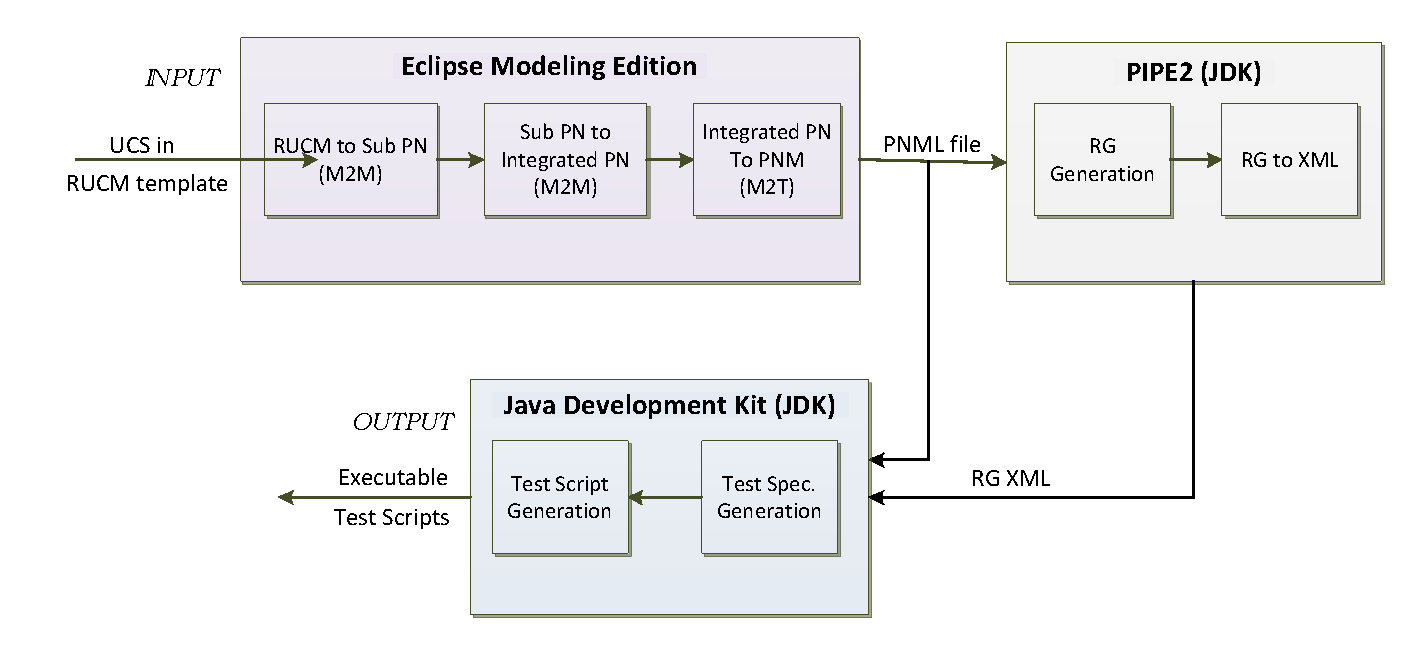
\includegraphics[width=1.05\textwidth]{content/images/Chapter5/SystemDesign}}
\caption{An overview of the different components in the tool}
\label{fig:systemdesign}
\end{figure}

Next important constraint is the need for an intermediate input artifact that describes the environment for which the test script has to be generated. In industry, usually the test scripts are implemented using tools and a mapping is needed to interface our implementation with the specific tool implementation.  Hence for this purpose, an implementation similar to a Lookup table is used in our tool design.

\subsection{System Design of the Tool}
Figure \ref{fig:systemdesign} shows the high level system design of the tool. The design tries to incorporate the design goals described in previous section taking into account the different limitations. The design can be divided into three blocks based on the platform on which they are implemented. The three blocks are implemented in Eclipse Modeling Edition, PIPE2 and \gls{jdk} respectively. The input of the system is \gls{ucs} in natural language and the output is the executable test scripts. Figure \ref{fig:systemdesign} also gives the details of different sub components in each block.

\section{Implementation of the Tool}
This section describes the implementation of various blocks defined in the previous section.

\subsection{Implementation in Eclipse Modeling Edition}
\subsubsection{Metamodels Developed}
This section explains in detail about the different metamodels that are developed for the implemention of the tool. The metamodels are developed using the Eclipse Modeling Project \cite{eclipse}.
\begin{figure}[htb!]
\centering
\fbox{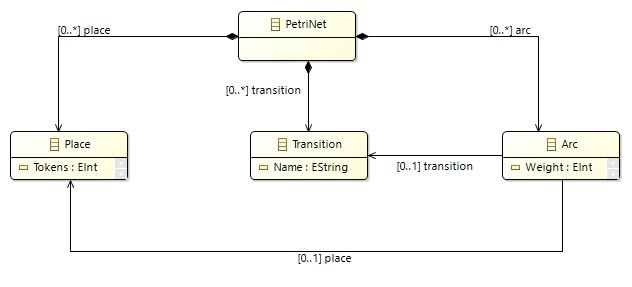
\includegraphics[width=1\textwidth]{content/images/Chapter5/PetriNetMetaModel}}
\caption{Petri Net Metamodel}
\label{fig:petrimetamodel}
\end{figure}

\begin{figure}[htb!]
\centering
\fbox{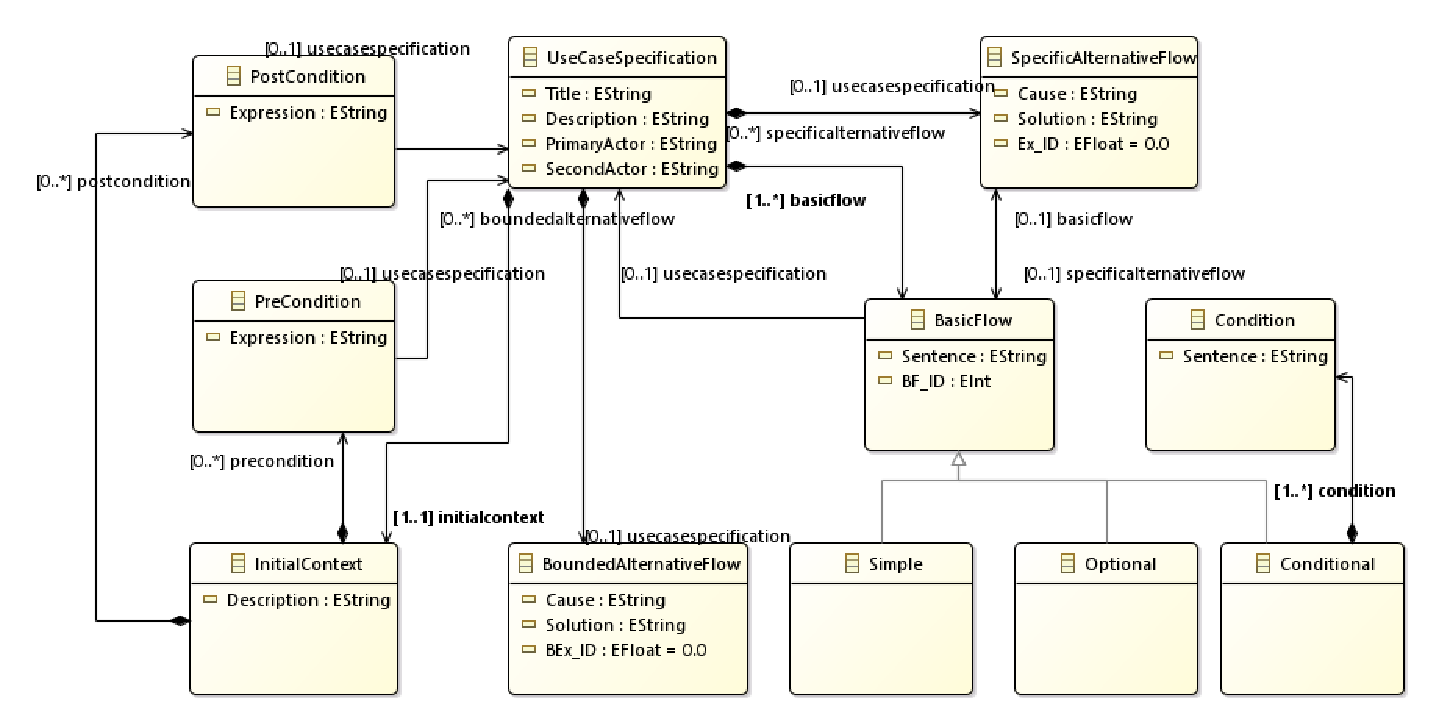
\includegraphics[width=1\textwidth]{content/images/Chapter5/UseCaseMetaModel}}
\caption{RUCM Metamodel}
\label{fig:rucmmetamodel}
\end{figure}

Petri Nets in our tool is based on the metamodel shown in Figure 1. As explained earlier, it consists of Places, Transitions and Arcs. 

The second metamodel developed is for the \gls{rnl} template. The \gls{rnl} used in our case is \gls{rucm} and the metamodel for its template is shown in Figure 2. Here some customization according to our design goals is made. The developed metamodel is a simplified version of the metamodel in \cite{yue2013facilitating} and models only the key features necessary for our tool. It is based more on the metamodel provided in \cite{calisaya2016analysis}. Some changes are made to the restriction rules such as the rule that mandates each alternative flow should begin with a conditional statement is added and the rule that mandates the presence of post condition in each basic flow is withdrawn. 

\subsubsection{Running Example}
The tool implementation described in the next sections is explained with the help of a running example. The system under consideration is \gls{lms} from Automotive Software. The \gls{lms} is used to enhance the safety of an automobile. The purpose of the system is to help the driver to keep the vehicle in their lane to avoid crashes. 

% Table generated by Excel2LaTeX from sheet 'Sheet1'
\begin{table}[htbp]
  \centering
  \caption{Running Example}
    \begin{adjustbox}{width=1\textwidth}
    \begin{tabular}{|l|l|l|l|l|l|l|l|}
    \toprule
    \textit{\textbf{Element}} & \multicolumn{7}{l|}{\textit{\textbf{ Description}}} \\
    \midrule
    \textbf{Use Case Name} & \multicolumn{7}{l|}{\textit{Disable System}} \\
    \midrule
    \textbf{Brief Description } & \multicolumn{7}{l|}{The LMS should be turned off at certain conditions.} \\
    \midrule
    \multirow{2}[4]{*}{\textbf{Precondition}} & \multicolumn{7}{l|}{1. LMS is activated} \\
\cmidrule{2-8}          & \multicolumn{7}{l|}{2. Vehicle Speed is greater than 15 kmph} \\
    \midrule
    \textbf{Primary Actor } & \multicolumn{7}{l|}{Driver, LMS Control Unit} \\
    \midrule
    \textbf{Secondary Actors} & \multicolumn{7}{l|}{LCS, LKS and LWKS Control Units} \\
    \midrule
    \multirow{6}[12]{*}{\textbf{Basic Flow}} & \multicolumn{7}{l|}{1. The driver deaccelerates the vehicle.} \\
\cmidrule{2-8}          & \multicolumn{7}{l|}{2. The driver accelerates the vehicle.} \\
\cmidrule{2-8}          & \multicolumn{7}{l|}{3. The driver drifts away from the current lane.} \\
\cmidrule{2-8}          & \multicolumn{7}{l|}{4. The driver activates the LKS system.} \\
\cmidrule{2-8}          & \multicolumn{7}{l|}{5. The LKS steers the vehicle.} \\
\cmidrule{2-8}          & \multicolumn{7}{l|}{6. The vehicle is moving through a road under repair.} \\
    \midrule
    \multicolumn{1}{|l|}{\multirow{4}[8]{*}{\textbf{Specific \newline{} Alternative Flows}}} & \multicolumn{7}{l|}{1.1 IF Vehicle Speed less than 15 kmph THEN deactivate LMS system with audio alert.} \\
\cmidrule{2-8}          & \multicolumn{7}{l|}{3.1 IF the departure is unintentional THEN create audio alert and deactivate LMS sytem.} \\
\cmidrule{2-8}          & \multicolumn{7}{l|}{5.1 IF the driver manually takes over THEN raise an alert and deactivate LKS.} \\
\cmidrule{2-8}          & \multicolumn{7}{l|}{6.1 IF the road markers are unclear THEN raise an alert and deactivate LMS} \\
    \bottomrule
    \bottomrule
    \end{tabular}%
    \end{adjustbox}
  \label{tab:runningexample}%
\end{table}%


The \gls{lms} consists of three main components namely a \gls{lcs}, a \gls{ldws} and a \gls{lks}. The \gls{ldws} alerts the driver in case of unintentional lane changes. The \gls{lcs} and \gls{lks} will work together to take control of the vehicle and keep the vehicle in driver defined center of the lane. Table 1 is an extract from the \gls{srs} document of \gls{lms} and it illustrates a specific Use Case called Disable System. The template used for specifying this Use Case is \gls{rucm} template and it is based on the metamodel described in the previous section.

\subsubsection{Input for \gls{tsgt}}
The next important step is to provide the input to the tool in the form of \gls{rucm} template. Once the input is entered, it should also be validated according to the template rules. For this, once the metamodels are developed, they should be exported as plug-ins and installed in the current host of Eclipse Modeling Edition.

\begin{figure}[htb!]
\centering
\fbox{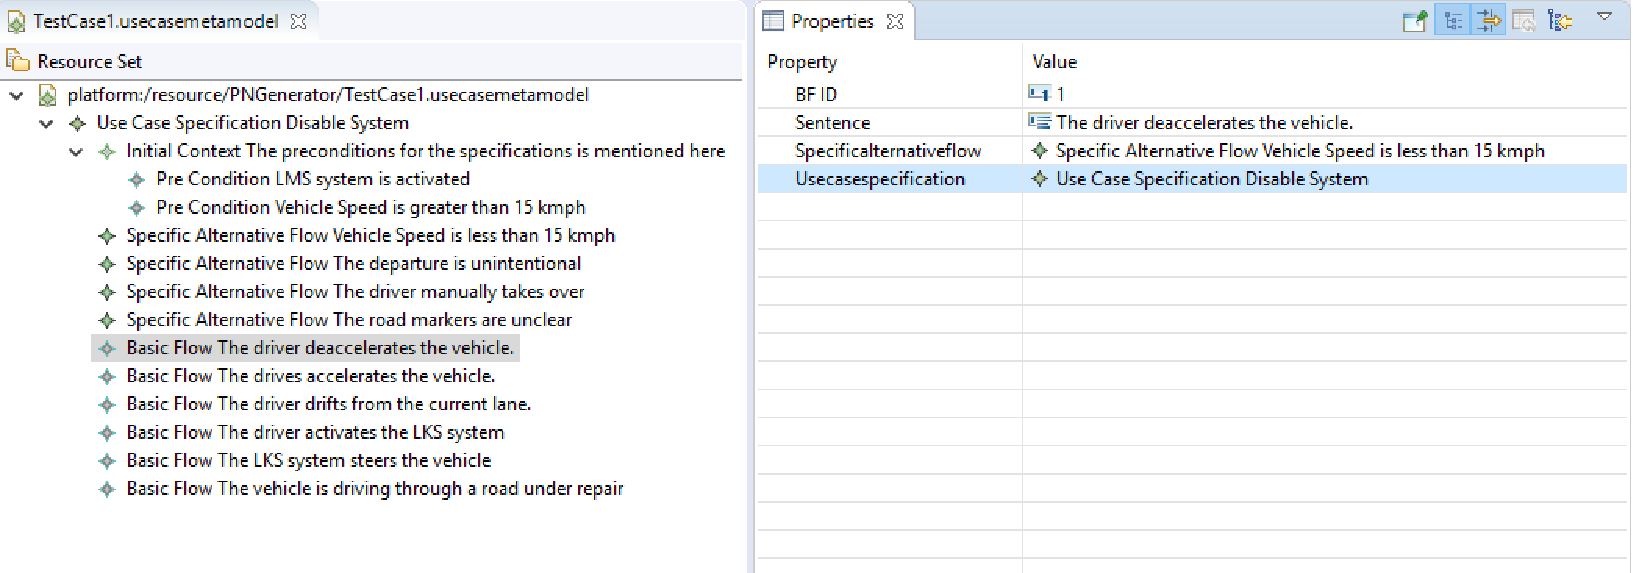
\includegraphics[width=1\textwidth]{content/images/Chapter5/Requiremens_Snip}}
\caption{Running example given as input to the tool}
\label{fig:input}
\end{figure}

\begin{figure}[htb!]
\centering
\fbox{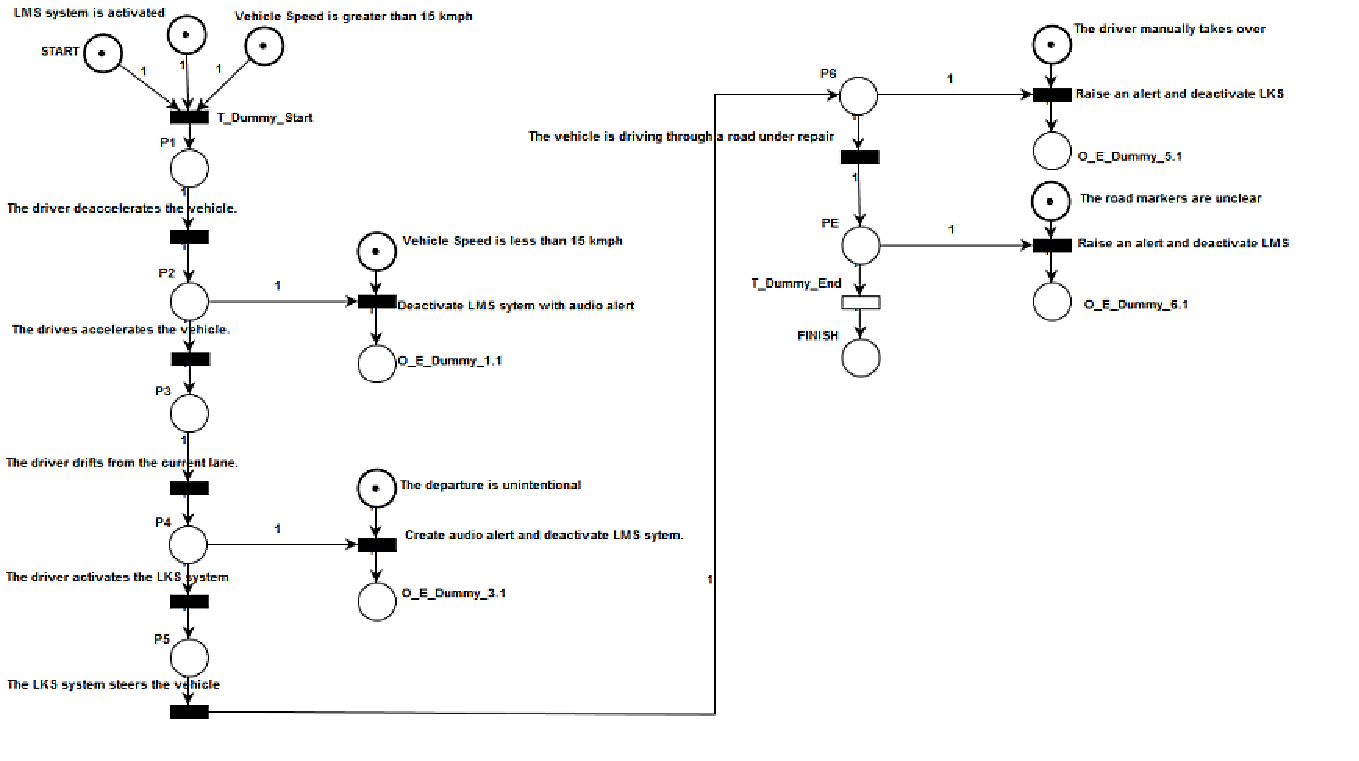
\includegraphics[width=1\textwidth]{content/images/Chapter5/FinalIntegratedPetriNet}}
\caption{Integrated Petri Net for the running example}
\label{fig:integratedpn}
\end{figure}


To give inputs to the tool, we should create an instance of the \gls{rucm} metamodel. The running example is given as input for the tool and the structure of the user input can be seen in the Figure 3.

\subsubsection{Model Transformations}
This section describes how the \gls{ucs} in \gls{rucm} metamodel is converted into an integrated Petri Net. Model transformations, which are the core of the MDSE technique, are used for this purpose.

The first step of the transformation process is to transform elements from \gls{rucm} metamodel to Petri Net metamodel elements. For this purpose, the concept of \gls{m2m} transformation is used and it needs specific rules for transformation from one metamodel to another.  In our tool, these rules are implemented using QVTo \cite{eclipseqvt}. Figure 4 gives a visual overview of the different transformation rules and Appendix xxx shows the precise implementation of the rules. 

Once this transformation is executed, we get a collection of Sub Petri Nets. These should be integrated again into a single Petri Net using the rules defined in section xxx. These rules are again implemented using QVTo as a \gls{m2m} transformation. Appendix xxx shows the implementation of these rules.

The output of the above transformation yields an integrated Petri Net. In order to make this output compatible with other Petri Net tools, the available Petri Net is converted into a standard xml file called \gls{pnml}PNML. This transformation from Petri Net metamodel to textual representation is done using \gls{m2t} transformation implemented in Xpand language \cite{eclipsem2t}. Appendix xxx gives the details of this implementation. A graphical representation of the intermediate output for our running example in PIPE2 tool is shown in Figure 5.

\subsection{Implementation in PIPE2 tool}
This block generates the reachability graph. The integrated Petri Net in the form of the xml file is given as input to the PIPE2 tool. From this, reachablibility graph is generated using the corresponding menu in the tool. In order to use this graph in the subsequent steps, it is exported as an xml file. For this, a package is added to the existing tool and this exports the xml file with the template shown in appendix xxx. The implementation is done using \gls{jdk}.

\subsection{Implementation in \gls{jdk} environment}
This block is responsible for the generation of test specifications and test scripts. Inputs to this section are the Reachability Graph and the \gls{pnml} file. The test specification is generated by identifying the reachable paths from the Reachability Graph and then the conditions from the \gls{pnml} file are added. For identifying all reachable paths, an \textit{All Path Search} is done from initial state to tangible states using \textit{Depth First Search Algorithm}.

\begin{figure}[htb!]
\centering
\fbox{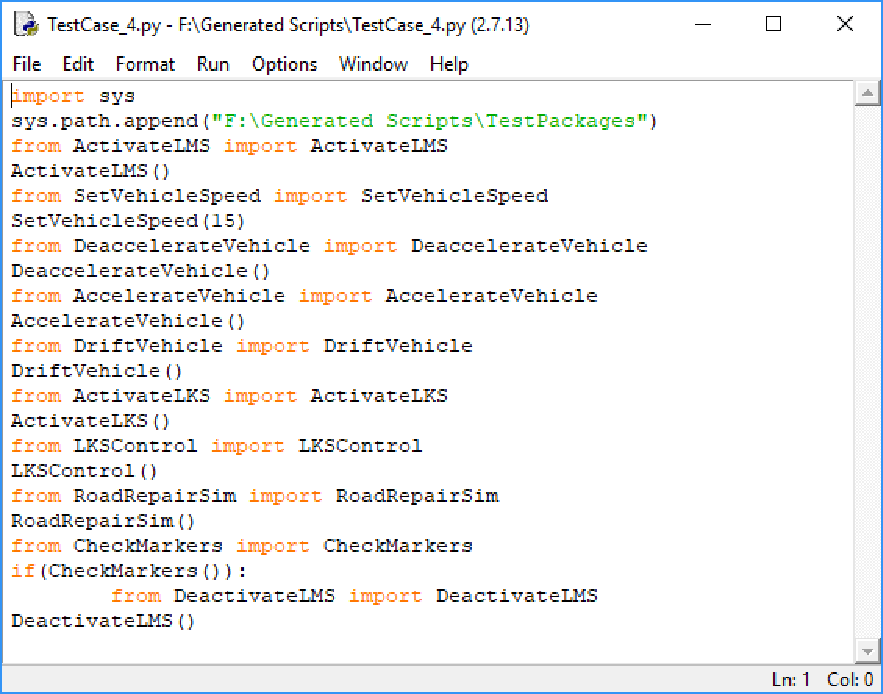
\includegraphics{content/images/Chapter5/TestScript}}
\caption{The final output of the TSTG tool}
\label{fig:testscript}
\end{figure}

Once a test specification is ready, each test case in the test specification is elicited out and the test steps for the test cases are generated using an implementation similar to Lookup table. This Lookup table maps each test step to a package predefined in python and finally executable test cases are generated in python. Figure x shows a generated test script for one of the test cases of our running example. The entire implementation is done in \gls{jdk} using Eclipse Java Standard Edition.
